\documentclass[UTF-8, a4paper, 12pt]{ctexart}

\usepackage[left=1in,right=1in,top=1.00in,bottom=1.00in]{geometry}% 页边距
\usepackage[colorlinks,linkcolor=blue,anchorcolor=blue,citecolor=green,CJKbookmarks=True]{hyperref}
\usepackage{CJK,CJKnumb}
\usepackage{indentfirst}        % 首行缩进宏包
\usepackage{latexsym,bm}        % 处理数学公式中和黑斜体的宏包
\usepackage{amsmath,amssymb}     % AMSLaTeX宏包 用来排出更加漂亮的公式
\usepackage{graphicx}
\usepackage{cases}
\usepackage{pifont}
\usepackage{txfonts}
\usepackage{subfigure}
\usepackage{pdfpages}
\usepackage{listings}
\usepackage{xcolor}
\usepackage[subfigure]{tocloft}     % 模板中用了subfigure,不加此选项会产生冲突
\usepackage{inconsolata}
\CTEXsetup[format={\Large\bfseries}]{section}%设置章标题字号为Large,居左
\zihao{-4}\linespread{1.5}\selectfont
\renewcommand{\theequation}{\arabic{section}-\arabic{equation}}
\renewcommand{\thefigure}{\arabic{section}-\arabic{figure}}
%\renewcommand{\thefigure}{\thechapter-\arabic{figure}}
\renewcommand{\cftsecleader}{\cftdotfill{\cftdotsep}}
\renewcommand\contentsname{{\qquad\qquad\qquad\qquad\qquad\qquad 目\quad 录}}
\newcommand{\song}{\CJKfamily{song}}    % 宋体   (Windows自带simsun.ttf)
\renewcommand{\abstractname}{\textbf{\large {摘\quad 要}}} %更改摘要二字的样式

%%%%%%%%%%%%%%%%%%%%%%%
% -- text font --
% compile using Xelatex
%%%%%%%%%%%%%%%%%%%%%%%
% -- 中文字体 --
%\setCJKmainfont{Microsoft YaHei}  % 微软雅黑
%\setCJKmainfont{YouYuan}  % 幼圆
%\setCJKmainfont{NSimSun}  % 新宋体
%\setCJKmainfont{KaiTi}    % 楷体
%\setCJKmainfont{SimSun}   % 宋体
%\setCJKmainfont{FangSong}   % 仿宋
%\setCJKmainfont{SimHei}   % 黑体
 
% -- 英文字体 --
%\setmainfont{Times New Roman}
%\setmainfont{DejaVu Sans}
%\setmainfont{Latin Modern Mono}
%\setmainfont{Consolas}
\setmainfont{CMU Serif}



%%%%%%%%%%%%%%%%%%%%%%%
%  设置水印
%%%%%%%%%%%%%%%%%%%%%%%
%\usepackage{draftwatermark}         % 所有页加水印
%\usepackage[firstpage]{draftwatermark} % 只有第一页加水印
%\SetWatermarkText{Copyright(C) 2021. by HU S K}           % 设置水印内容
% \SetWatermarkText{\includegraphics{fig/ZJDX-WaterMark.eps}}         % 设置水印logo
%\SetWatermarkLightness{00.9}             % 设置水印透明度 0-1
%\SetWatermarkScale{0.4}                   % 设置水印大小 0-1
%%%%%%%%%%%%%%%%%%%%%%%




%%%%%%%%%%%%%%%%%%%%%%%%%%%%%%%%%%%%%%%%%%%
%用来设置附录中代码的样式
% 头文件
%%%%%%%%%%%%%%%%%%%%%%%%%%%%%%%%%%%%%%%%%%%
\usepackage{listings} 
\usepackage{fontspec}
\setmonofont{Consolas}
%\begin{lstlisting}[
%	language = matlab, numbers=left, 
%	numberstyle=\tiny,keywordstyle=\color{blue!70},
%	commentstyle=\color{red!50!green!50!blue!50},frame=shadowbox,
%	rulesepcolor=\color{red!20!green!20!blue!20},
%	basicstyle=\ttfamily,
%	]
%	
%\end{lstlisting}



\title{\bfseries \Huge  }
\author{H.S.K.}
\date{}

\begin{document}
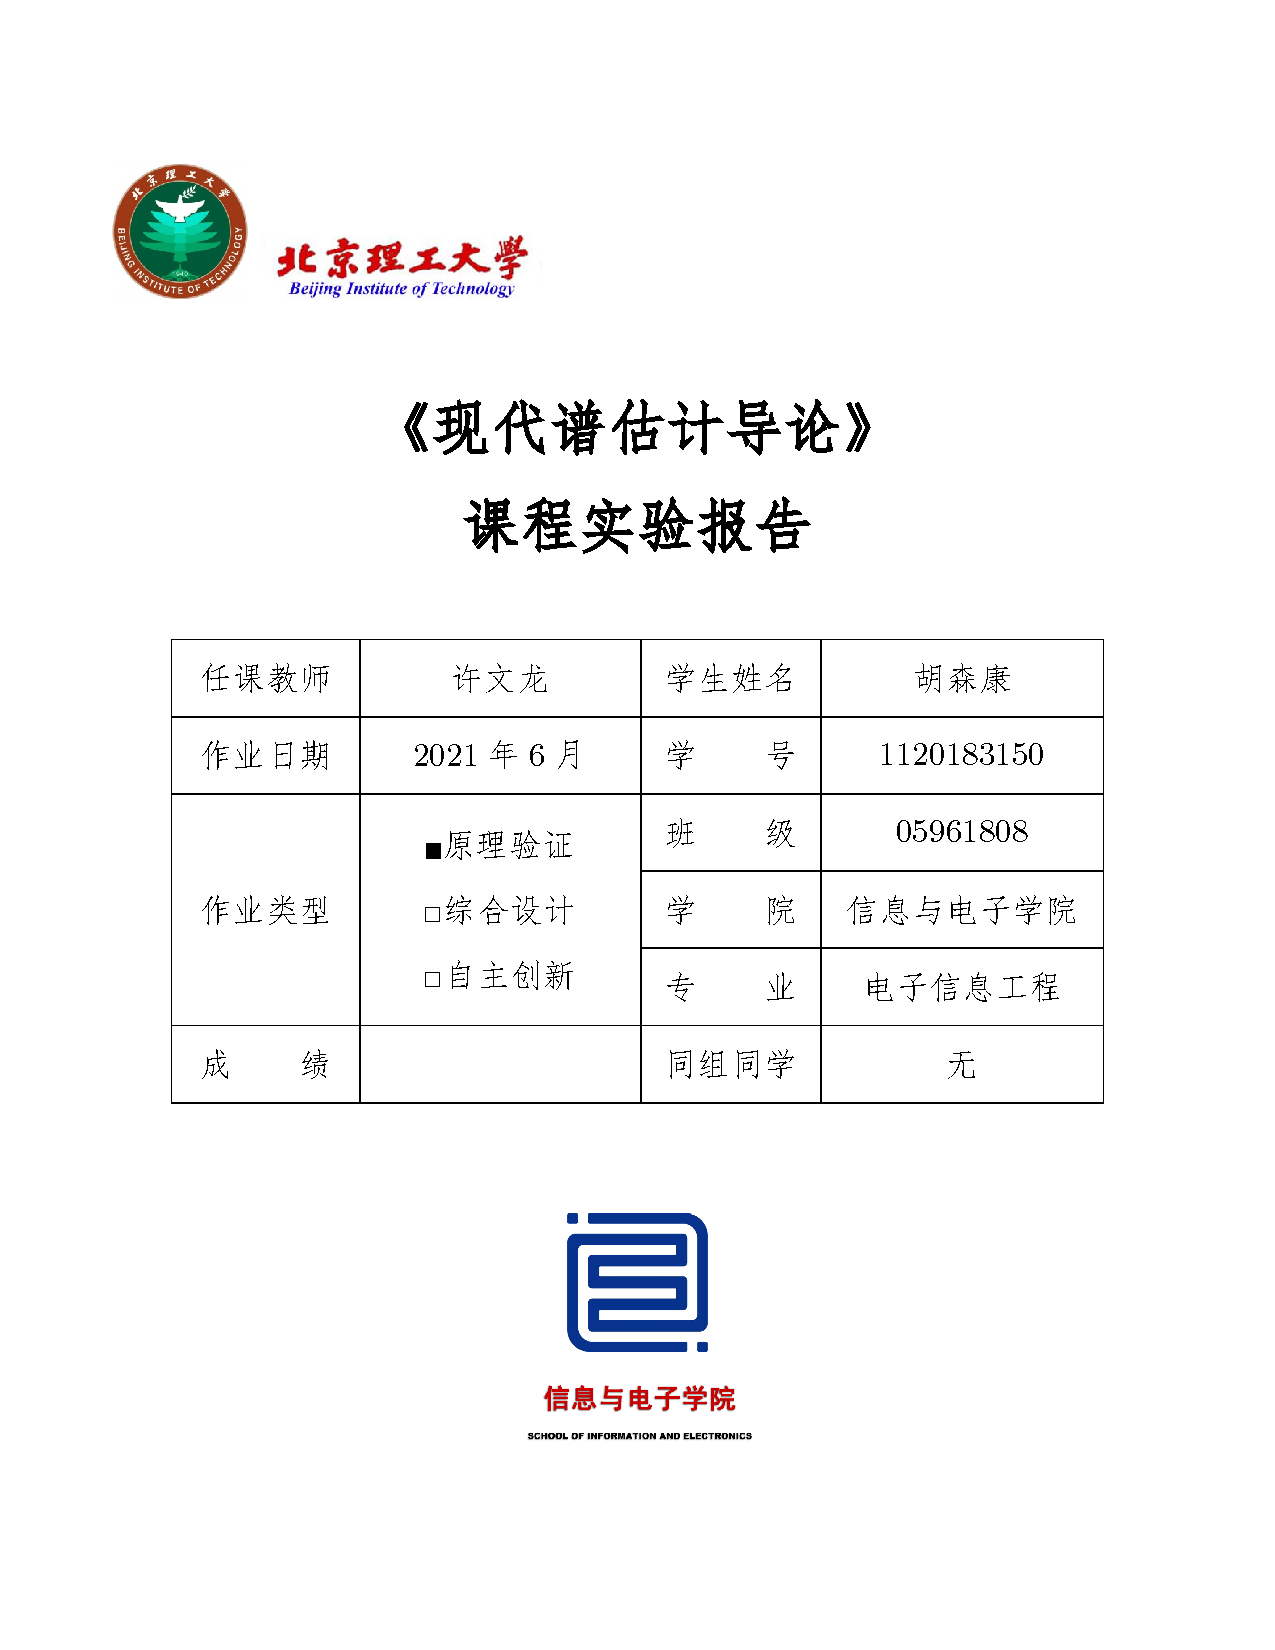
\includepdf[pages={1}]{coverpage.pdf} %% 插入pdf

%\maketitle

%\thispagestyle{empty}
%\newpage
%\thispagestyle{empty}
%\begin{abstract}
    %这里是中文摘要。这里是中文摘要。这里是中文摘要。这里是中文摘要。这里是中文摘要。这里是中文摘要。这里是中文摘要。这里是中文摘要。这里是中文摘要。这里是中文摘要。这里是中文摘要。这里是中文摘要。这里是中文摘要。这里是中文摘要。这里是中文摘要。这里是中文摘要。
 

%\end{abstract}

     

     
%\thispagestyle{empty}       %本页不显示页码
%\newpage                    %分页
\tableofcontents\thispagestyle{empty}
\newpage
\setcounter{page}{1}        %从下面开始编页,页脚格式为导言部分设置的格式



\section{C1.12 用计算机产生自协方差序列}

\subsection{Question Statement}
自协方差序列是双边序列。本题研究利用计算机产生双边ACS。


设$y(t)$为图(\ref{filter})所示线性系统的输出。系统的传输函数$H(z)=\frac{1+b_1z^{-1}}{1+a_1z^{-1}}$,输入是均值为0,方差为$\sigma^2$的白噪声信号。
\begin{figure}[htbp]
    \centering
    
\includegraphics[width=10cm]{fig/f1.png}
    \caption{线性系统的输入与输出PSD之间的关系}
    \label{filter}
\end{figure}

(a) 以$a_1$,$b_1$和$\sigma^2$为参数,求$r(k)$的解析解。

(b) $-20\leq k\leq 20$时,画出$r(k)$在$a_1$和$b_1$取不同值时的图形,注意$r(k)$拖尾的衰减速度与$|a_1|$有关。

(c) 当$a_1 \simeq b_1$,$\sigma^2=1$时,$r(k)\simeq \delta_{k,0}$。用$a_1=-0.95$,$b_1=-0.9$, 和$c_1=-0.7$验证上述结果。

(d) 在计算机上(近似地)产生$r(k)$的快速方法是利用$r(k)=\sigma^2h(k)*h^*(-k)$,其中$h(k)$是图(\ref{filter})中滤波器的冲激响应,$*$表示卷积运算。考虑:
\begin{equation}
    H(z)=\frac{1+b_1z^{-1}+\cdots+b_mz^{-m}}{1+a_1z^{-1}+\cdots+a_mz^{-m}}
\end{equation}
编写一个名为genacs.m的MATLAB函数,输入为$M$,$\sigma^2$,$a$,$b$,其中$a$和$b$分别为分母和分子的系数,输出是$0\sim M$对应的ACS系数矢量。编写的函数应该使用MATLAB函数filter(用来产生$\{h_k\}^M_{k=0}$)和conv(用来利用截断的冲激响应序列计算$r(k)=\sigma^2h(k)*h^*(-k)$)。

(e)用$\sigma^2=1$,$a_1=-0.9$,$b_1=0.8$测试所编写的函数,$M$分别为20和150;为什么$M$值较大时计算结果更精确?建议给出一个与滤波器极点相关的选取$M$的“经验法则”。
\subsection{Solution}

\subsubsection{The Solution of (a)}
We have $\phi_y(\omega)=|H(\omega)|^2\phi_e(\omega)$, Thus:
\begin{align}
     \phi_y(\omega) & = \frac{\sigma(1+b_1e^{-j\omega})(1+b_1^*e^{j\omega})}{(1+a_1e^{-j\omega})(1+a_1^*e^{j\omega})}   \\
     &=\frac{\sigma^2(1+|b_1|^2+b_1e^{-j\omega}+b_1^*e^{j\omega})}{(1+a_1e^{-j\omega})(1+a_1^*e^{j\omega})}
\end{align}

We use the following DTFT pair (for $|\alpha|$<1):
\begin{equation}
    c(k)=\left\{\begin{array}{ll}
        \alpha^k,& k\geq 0\\
        (\alpha^*)^{-k},&k<0
    \end{array}\right.\Longleftrightarrow C(\omega)=\frac{1-|\alpha|^2}{(1-\alpha^{-j\omega})(1-\alpha^*e^{j\omega})}
\end{equation}

We thus have:
\begin{equation}
    r(k)=\frac{\sigma^2}{1-|a_1|^2}\left[b_1d_{k-1}+(1+|b_1|^2)d_k+b_1^*d_{k+1}\right]
\end{equation}
where
\begin{equation}
    d(k)=\left\{\begin{array}{ll}
        (-a_1)^k,&k\geq0\\
        (-a_1^*)^{-k},&k<0
    \end{array} \right.
\end{equation}
\subsubsection{The Solution of (b)}

We use the MATLAB to generate the $r(k)$, and use the different $a_1$ and $b_1$, we can see the graphs of $r(k)$ from the following pictures.

\begin{figure}[htbp]
    \centering
    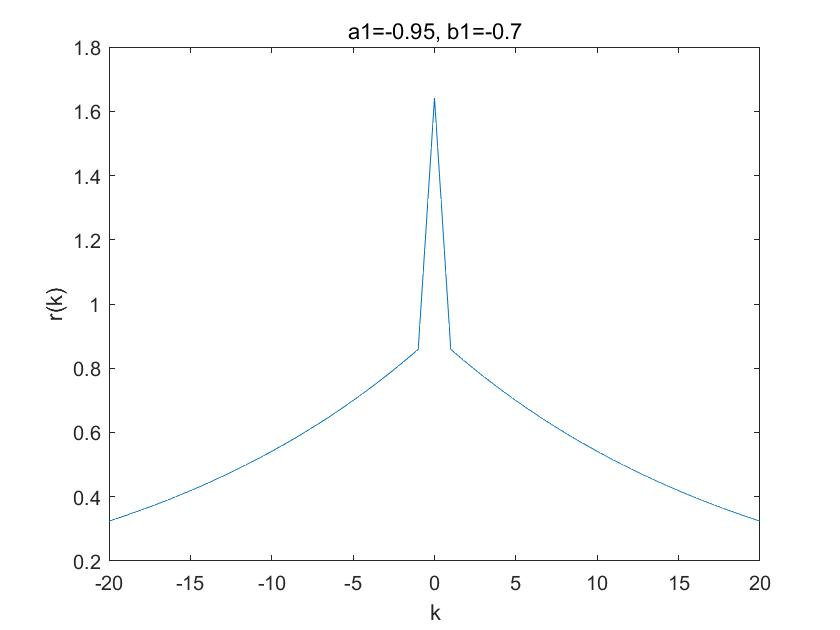
\includegraphics[width=7.5cm]{1/f1.jpg}
    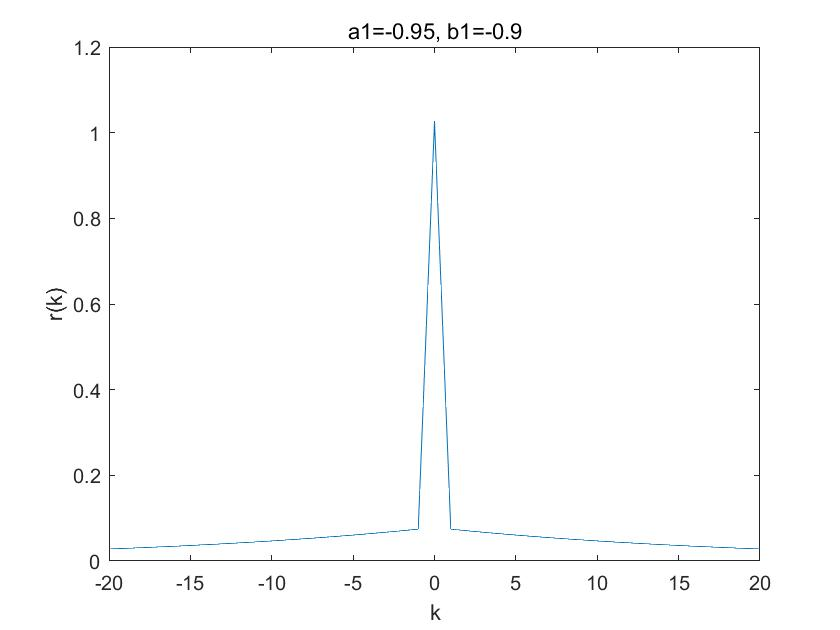
\includegraphics[width=7.5cm]{1/f2.jpg}
    \caption{The  graphs of $r(k)$ with different $a_1$ and $b_1$}
    \label{f1}
\end{figure}
\begin{figure}[htbp]
    \centering
   
    
    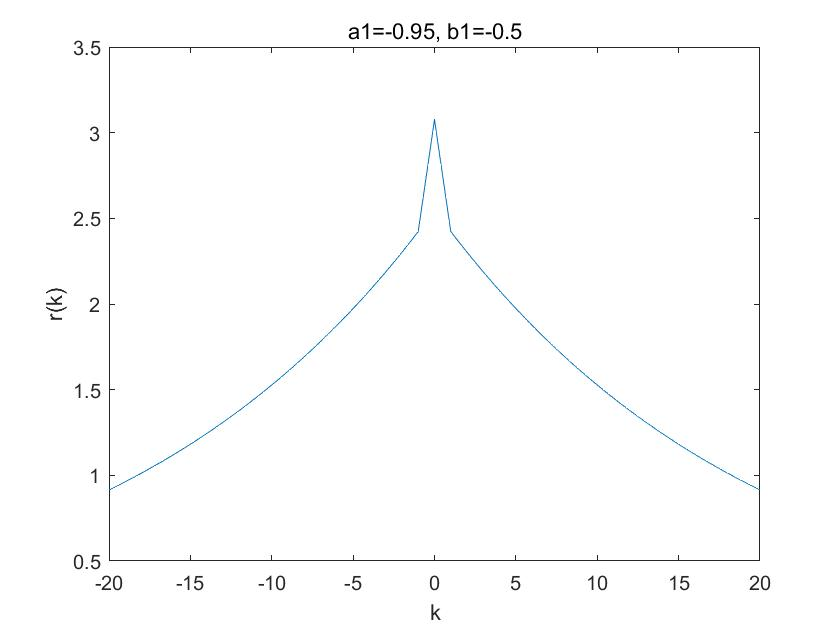
\includegraphics[width=7.5cm]{1/3.jpg}
    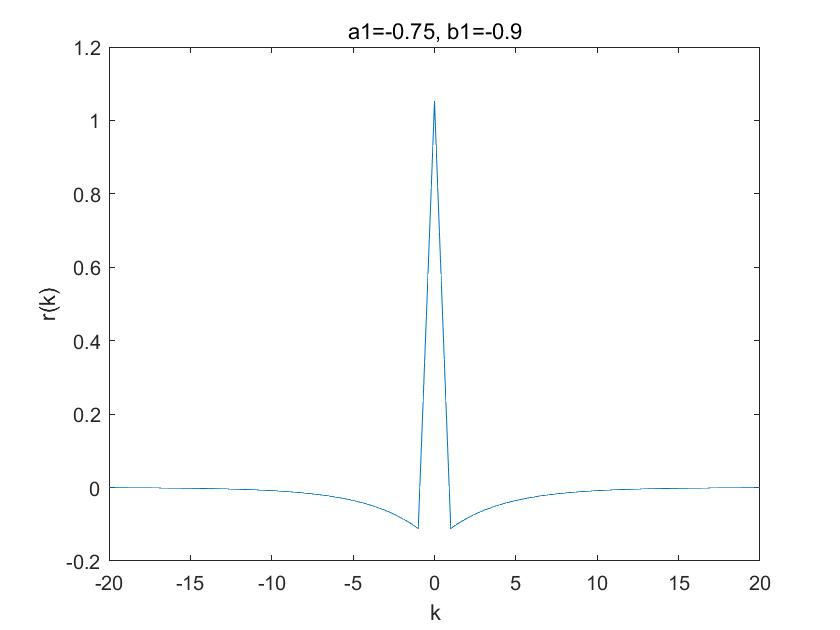
\includegraphics[width=7.5cm]{1/4.jpg}
    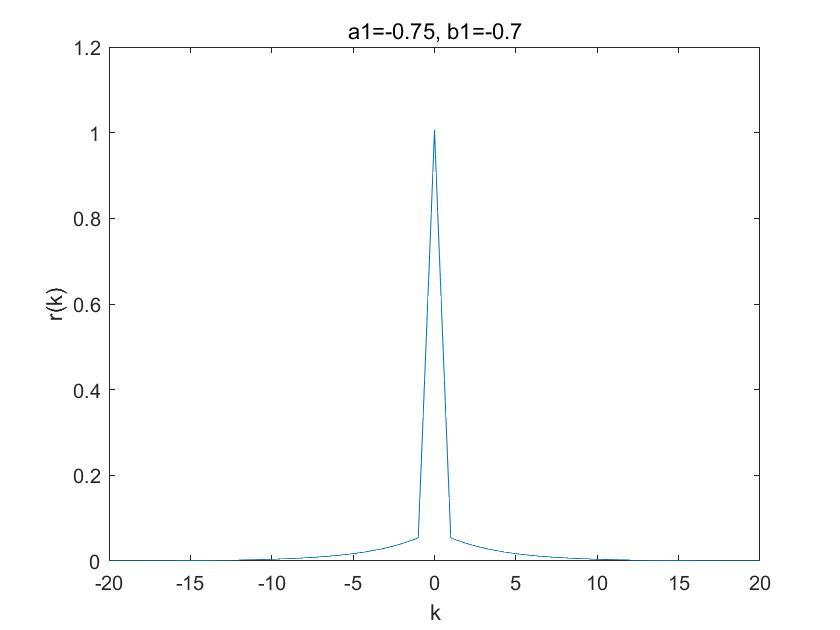
\includegraphics[width=7.5cm]{1/5.jpg}
    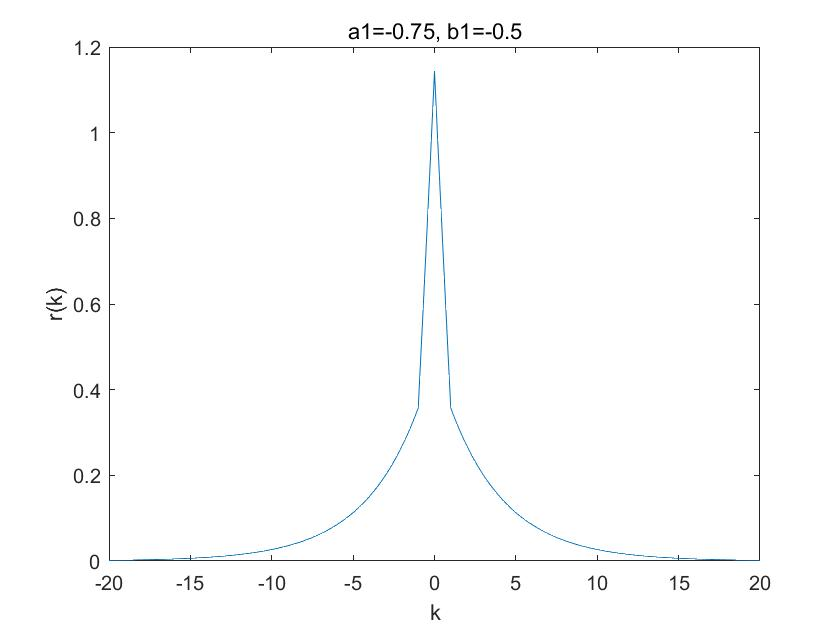
\includegraphics[width=7.5cm]{1/6.jpg}
    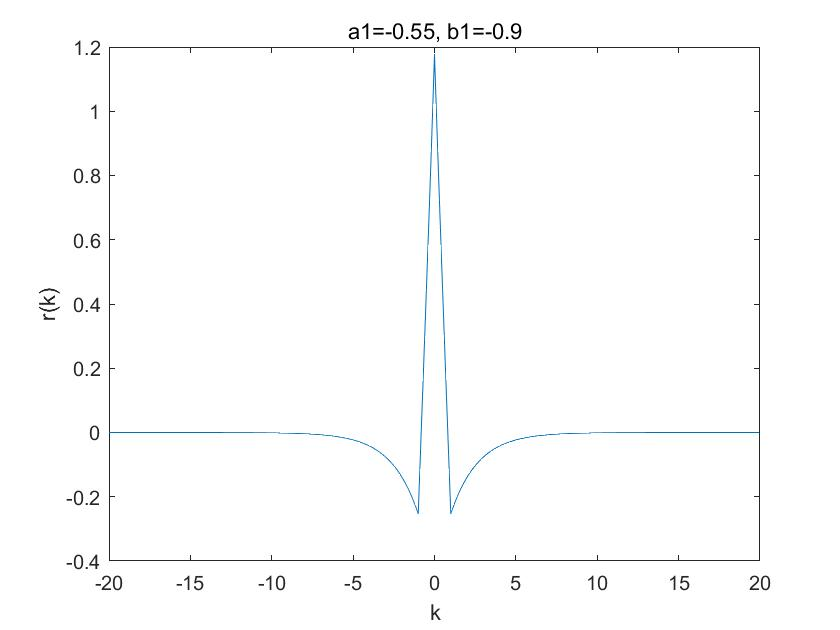
\includegraphics[width=7.5cm]{1/7.jpg}
    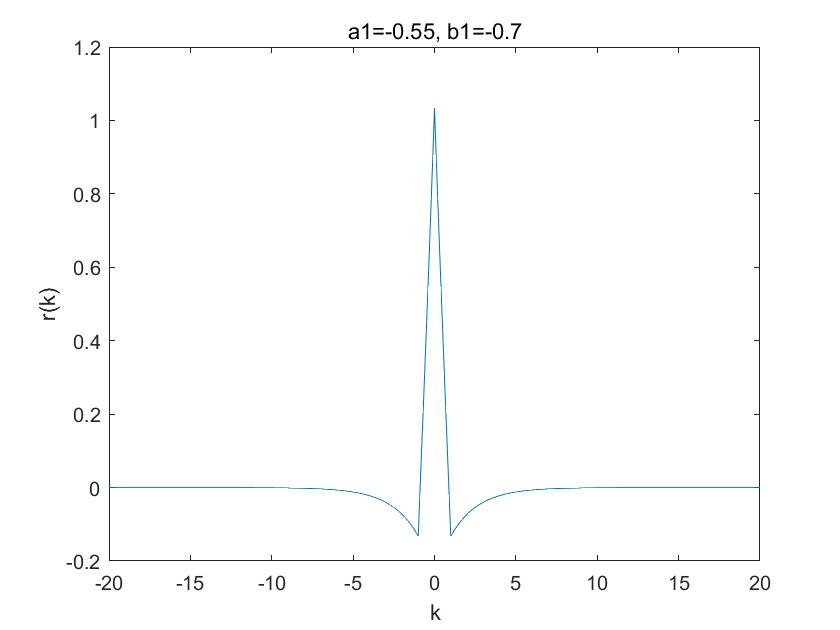
\includegraphics[width=7.5cm]{1/8.jpg}
    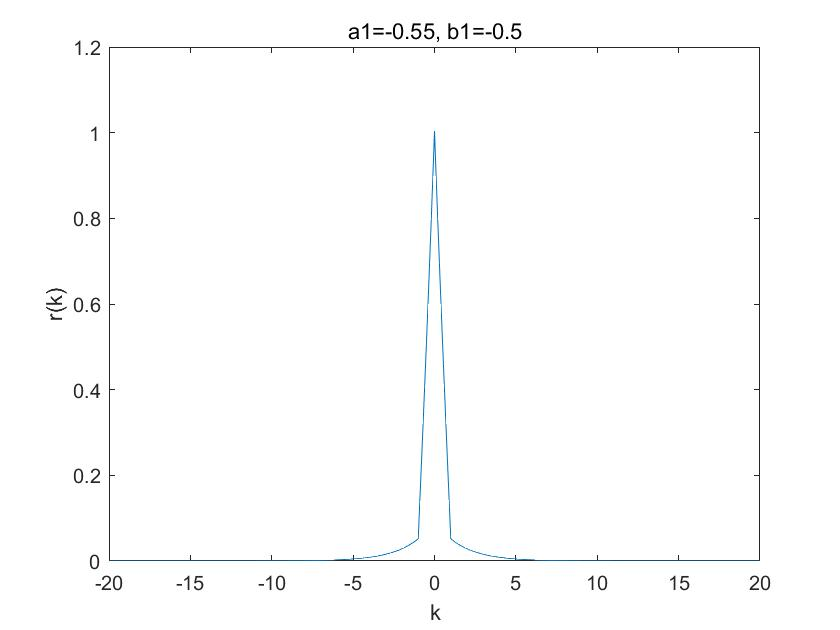
\includegraphics[width=7.5cm]{1/9.jpg}
    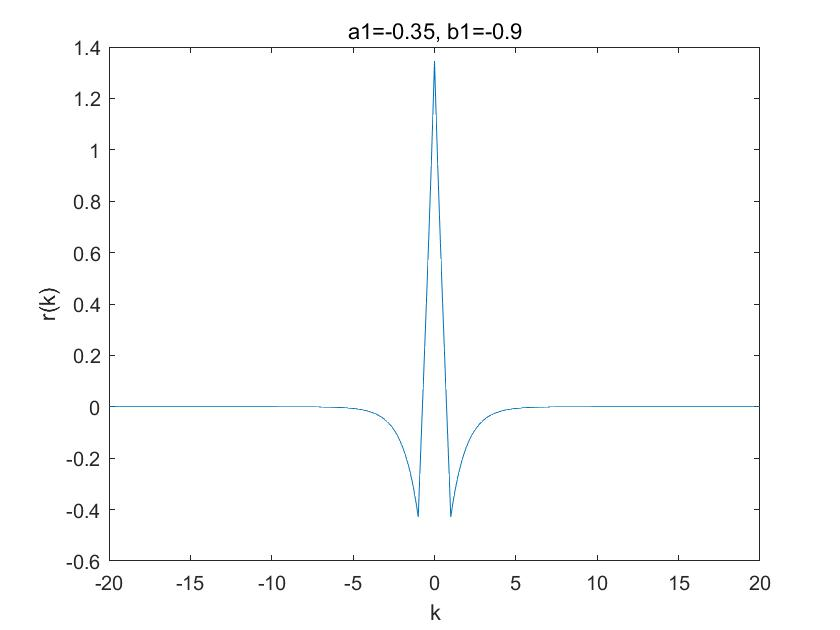
\includegraphics[width=7.5cm]{1/10.jpg}
    \caption{The  graphs of $r(k)$ with different $a_1$ and $b_1$}
\end{figure}
\begin{figure}[htbp]
    \centering
    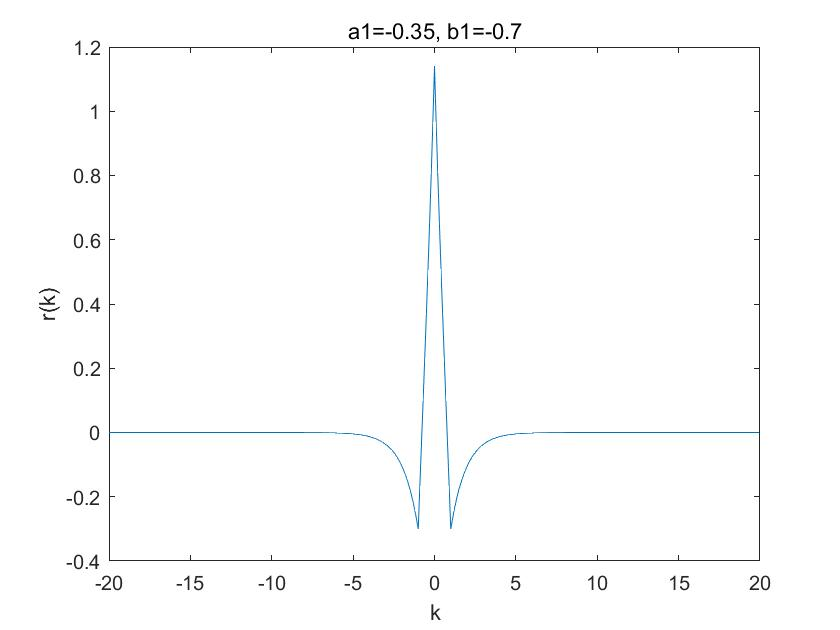
\includegraphics[width=7.5cm]{1/11.jpg}
    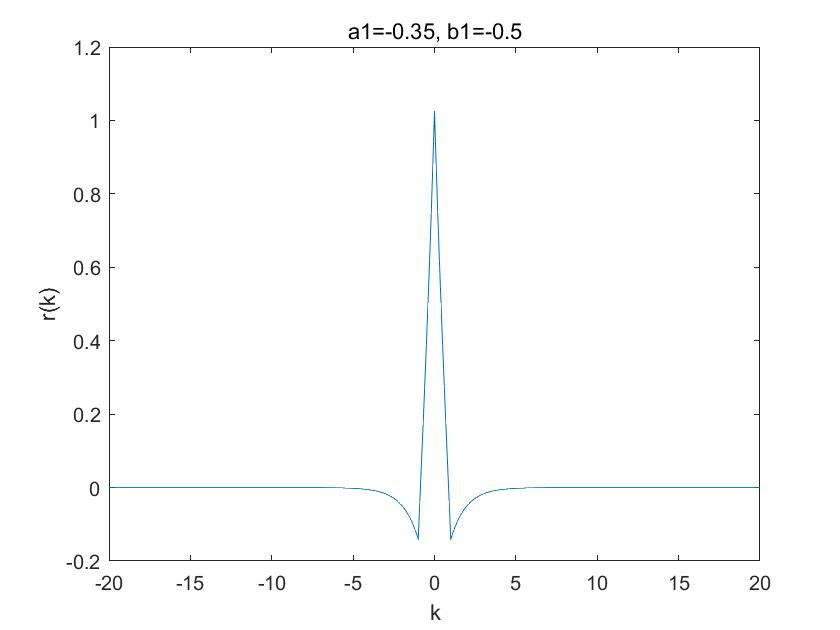
\includegraphics[width=7.5cm]{1/12.jpg}
    \caption{The  graphs of $r(k)$ with different $a_1$ and $b_1$}
\end{figure}

\newpage
\subsubsection{The Solution of (c)}

From the Figure (\ref{f1}), we can know that when $a_1\simeq b_1$, then $r_k\simeq\delta_{k,0}$.

\subsubsection{The Solution of (d)}

The function is very easy to write by MATLAB, and I can write this function by the following program:
\begin{lstlisting}[
	language = matlab, numbers=left, 
	numberstyle=\tiny,keywordstyle=\color{blue!70},
	commentstyle=\color{red!50!green!50!blue!50},frame=shadowbox,
	rulesepcolor=\color{red!20!green!20!blue!20},
	basicstyle=\ttfamily,
	]
function acs=genacs(M, sigma, a, b)
h = filter([1;b(:)],[1,a(:)],[1;zeros(M,1)]);
acs = sigma*conv(h,flipud(conj(h)));
plot(acs);
\end{lstlisting}

\subsubsection{The Solution of (e)}

By using the 'genacs.m' MATLAB function, we get the impulse response of the filter in Figure (\ref{filter}), we can see the impulse response by the following pictures with $M=20$ and $M=150$, respectively.
\begin{figure}
    \centering
    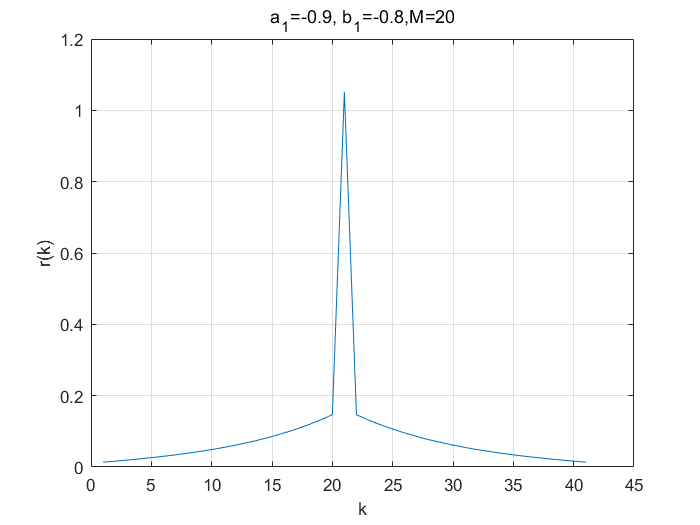
\includegraphics[width=7.5cm]{1/e1.png}
    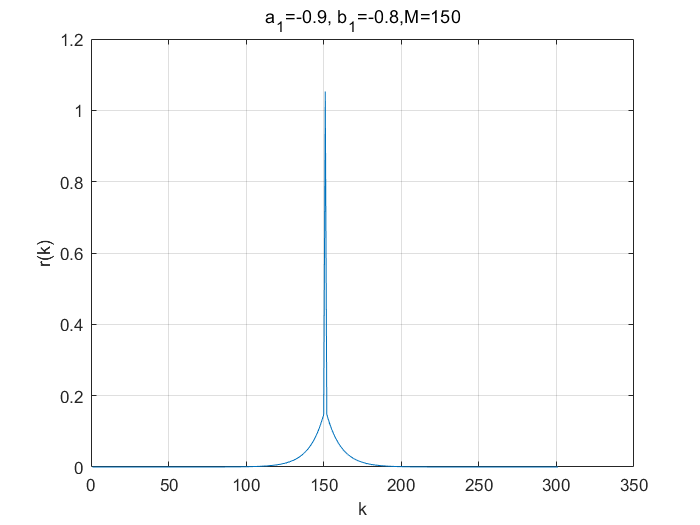
\includegraphics[width=7.5cm]{1/e2.png}
    \caption{$M=20$ and $M=150$, respectively}
\end{figure}


\newpage
\section{C2.20 周期图的分辨率和泄露特性}

\subsection{Question Statement}

由2.4节可知,周期图的期望值是真实频谱$\phi_y (\omega) $和Bartlett窗的傅里叶变换$W_B(\omega)$的卷积。$W_B(\omega)$函数的形状和长度决定了周期图平滑和泄漏的程度。同样,在式(2.6.24)中引入了加窗的周期图,其期望值等于Blackman-Tukey估计器的期望值,Blackman-Tukey估计器的加权值$w(k)$由式(2.6.31)给出。周期图估计中能够使用与矩形窗不同的窗函数,相关图估计也是如此。窗函数的选择会影响周期图(相关图)估计的分辨率和泄漏特性。
\newline

{\bfseries 分辨率特性}:谱估计的平滑度由窗的主瓣宽度决定,频谱泄漏量由副瓣的能量决定。平滑度限制了周期图的分辨率,下面用实例进行研究。

首先通过两个频率很“近”的被噪声污染的正弦序列来研究分辨率特性。考虑:
\begin{equation}
    y(t)=a_1\sin(f_0\cdot 2\pi t+\phi_1)+a_2\sin((f_0+\frac{\alpha}{N})2\pi t+\phi_2)+e(t)
\end{equation}
其中$e(t)$是均值为零,方差为的实高斯白噪声。这里令$f_0=0.2$,$N = 256$,但结果几乎与$f_0$和$N$无关。

(a)求出$W_B(\omega)$主瓣的3 dB带宽,$N$为参数,并验证式(2.4.18);计算副瓣峰值高度(dB),$N$为参数。注意窗函数的副瓣大小通常与$N$无关。取几个不同$N$值画出$W_B(\omega)$幅度图形,验证此结论,画图时分别采用线性和分贝坐标。

(b)令$\sigma^2=0$(消除周期图的统计方差,以便单独研究偏差特性),并令$a_1= a_2=1$和$\phi_1=\phi_2=0$。对于不同的$\alpha$,画出$y(t)$的(补零后)周期图图形,确定分辨率的阈值(即可以分开两个频率分量的最小$\alpha$值)。该值与2.4节中预测的分辨率相比如何?

(c)对加Hamming 窗的相关图估计重复(b)。

(d)对于理想的高信噪比(signal-to-noise ratio, SNR)和幅度相近的信号来说,(b)和(c)的分辨率阈值对信号幅度和频率$f_0$的变化不敏感。但这些阈值对相位$\phi_1$和$\phi_2$是敏感的,尤其当$\alpha$小于1时。试用两对($\phi_1$,$\phi_2$),使两个正弦信号在观察间隔的中心点分别同相和反相,比较它们的分辨率阈值;再用不同的$a_1$,$a_2$和$\sigma^2$值,验证它们对分辨率阈值的影响相对较小。\newline

{\bfseries 频谱泄漏}:这部分分析周期图估计的泄漏效应。当对两个幅度相差很大且完全分开的正弦信号进行估计时,可以清楚地看到泄漏效应。

(a)产生一个正弦序列,$ a =4, \sigma_2=0,\phi_1=\phi_2=0$。令$a_1 = 1$,改变$a_2$(例如$a = 1,0.1,0.01,0.001$)。计算周期图(选用矩形数据窗),分析用谱估计分辨第二个正弦信号的能力。

(b)对$\alpha = 12$重复(a)。分辨出第二个正弦信号的幅度阈值改变吗?

(c)观察$\alpha=4$和$\alpha= 12$时 Bartlett窗的傅里叶变换在频率$\alpha/N$处的幅度,解释(a)和(b)的结果。

(d)由(a)和(b)可知 , Bartlett窗的泄漏程度取决于数据中两频谱分量的距离(其他一些窗也一样)。在很多实际应用中,数据中正弦分量的动态范围可能已知,这时就需要用户选择副瓣电平具有等幅特性的窗。Chebyshev窗是一个很好的选择,因为用户在设计窗时可以选择(恒定的)副瓣电平(参见MATLAB命令chebwin)。

假设正弦分量的最大动态范围为60 dB。用式(2.6.31)设计一个Chebyshev窗$v( t)$和对应的 Blackman-Tukey 窗$w(k),$使下面的谱估计器可以在这个动态范围内将两个正弦分量分开:(i)窗为$w(k)$的 Blackman-Tukey谱估计器,(ii)窗为$v(t)$的加窗周期图。画出窗的傅里叶变换并确定它的频谱分辨率。

通过计算两个正弦信号的 Blackman-Tukey估计和加窗周期图估计,测试所设计的窗,其中这两个正弦信号幅度差的动态范围为50 dB且频率分开值为预测的最小值。将得到的分辨率与预测值进行比较。解释为什么利用其中的一种方法可以检测到幅度较小的正弦信号,另一种则不能。

\subsection{The Feature of Resolution}
\subsubsection{The Solution of (a)}
We have the result of the experiment:
\begin{figure}[htbp]
    \centering
    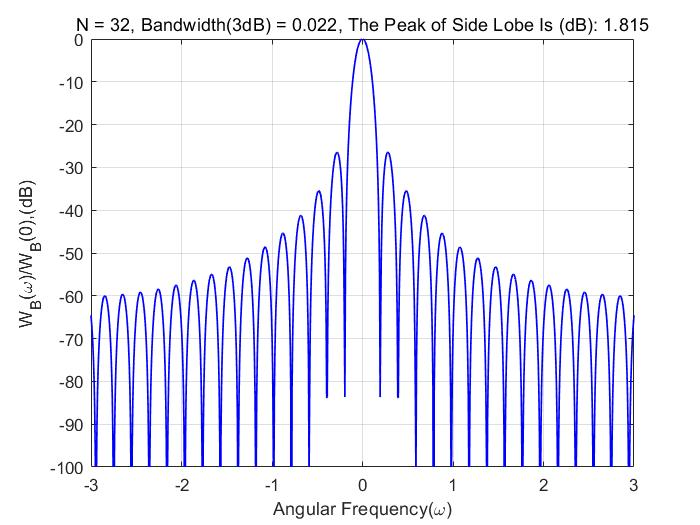
\includegraphics[width=7.5cm]{2/N32.jpg}
    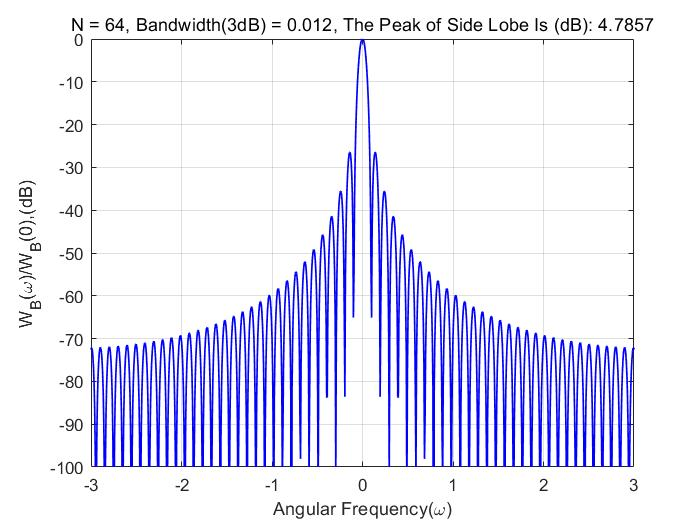
\includegraphics[width=7.5cm]{2/N64.jpg}
    \caption{The Bandwidth and the Peak of Sidelobe of $W_B(\omega)$ with $N=32, 64$}
\end{figure}
\begin{figure}[htbp]
    \centering
    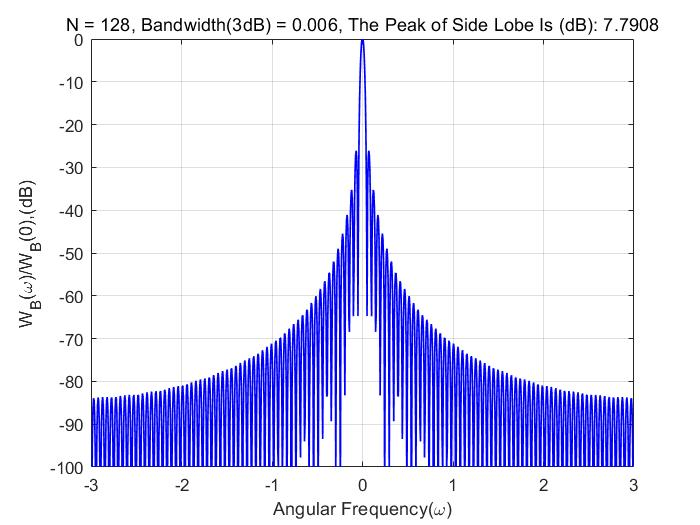
\includegraphics[width=7.5cm]{2/N128.jpg}
    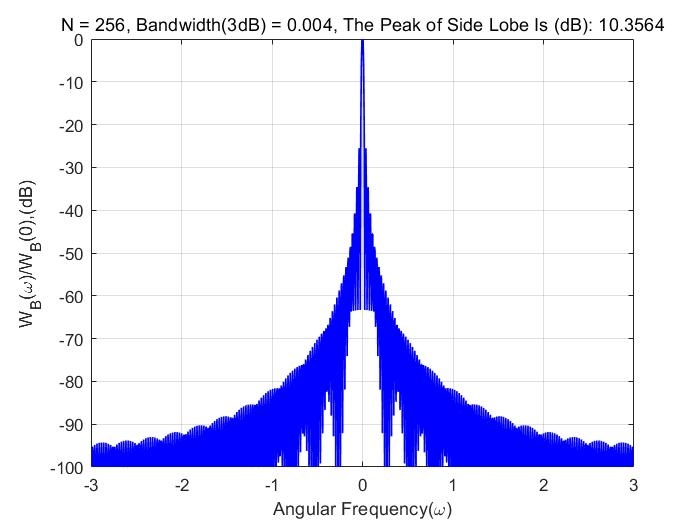
\includegraphics[width=7.5cm]{2/N256.jpg}
    \caption{The Bandwidth and the Peak of Sidelobe of $W_B(\omega)$ with $N=128, 256$}
\end{figure}

From the above plots, we see that the 3dB width is about $0.9\cdot\frac{2\pi}{N}$, and that the sidelobe level is essentially independent of N.

\subsubsection{The Solution of (b)}
We have the result of the experiment:
\begin{figure}[htbp]
    \centering
    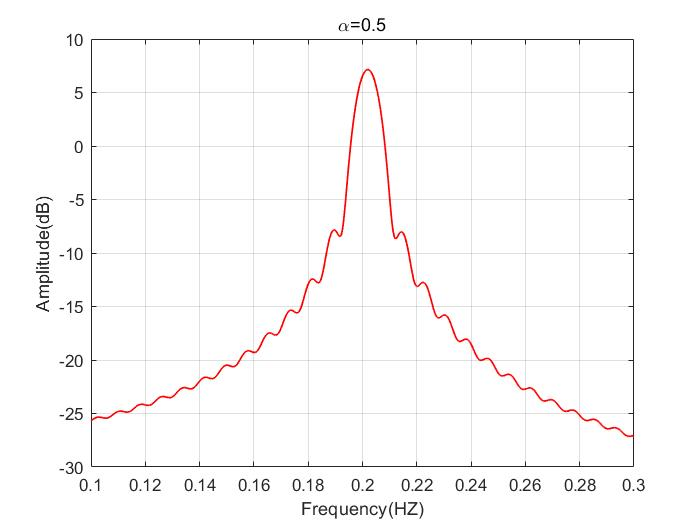
\includegraphics[width=7.5cm]{2/alpha05.jpg}
    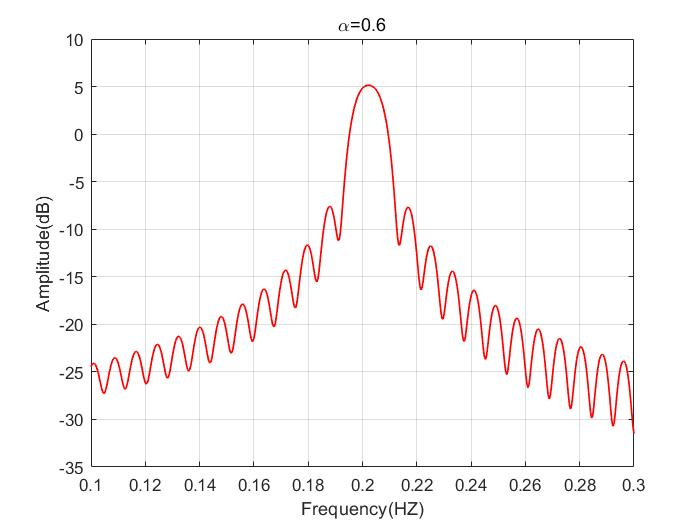
\includegraphics[width=7.5cm]{2/alpha06.jpg}
    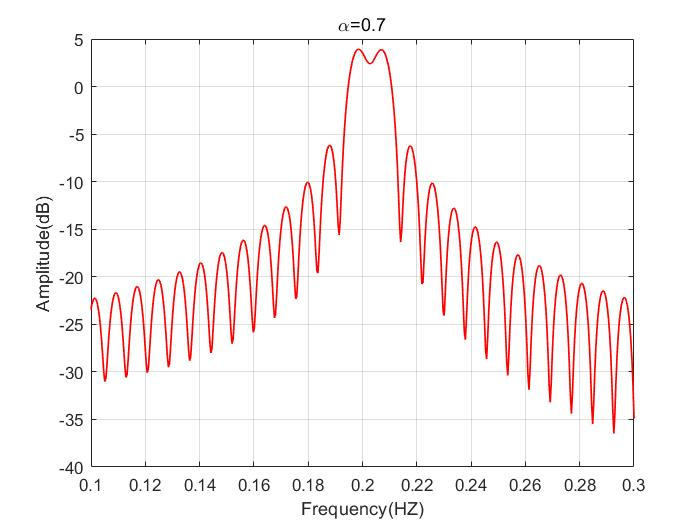
\includegraphics[width=7.5cm]{2/alpha07.jpg}
    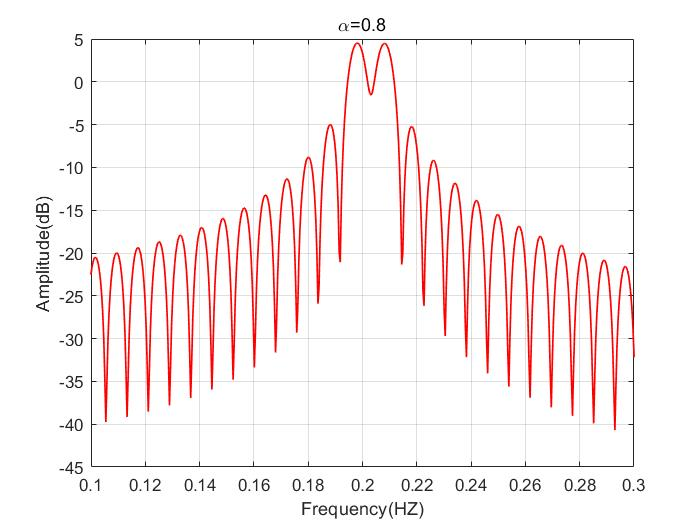
\includegraphics[width=7.5cm]{2/alpha08.jpg}
    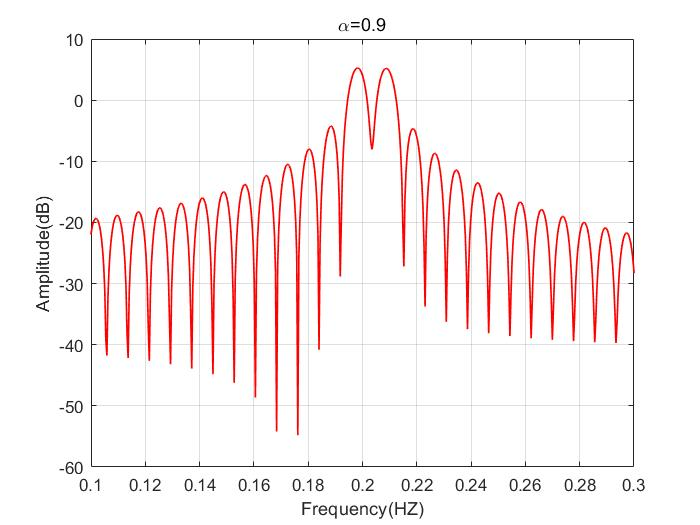
\includegraphics[width=7.5cm]{2/alpha09.jpg}
    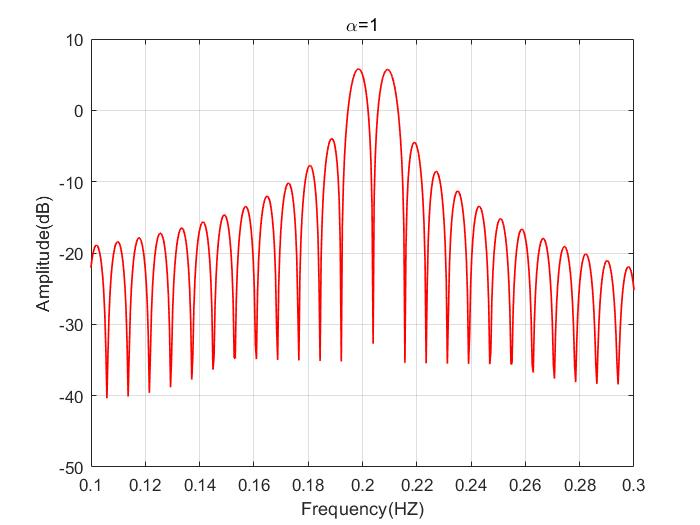
\includegraphics[width=7.5cm]{2/alpha10.jpg}
    \caption{$\alpha=0.5, 0.6, 0.7, 0.8, 0.9, 1.0$}
\end{figure}

We see the threshold $\alpha$ is about 0.7, giving a resolution of about $0.7\cdot\frac{2\pi}{N}$, which agrees with the $\simeq \frac{2\pi}{N}$ value stated in Section 2.4.

\subsubsection{The Solution of (c)}
We have the result of the experiment:
\begin{figure}[htbp]
    \centering
    
    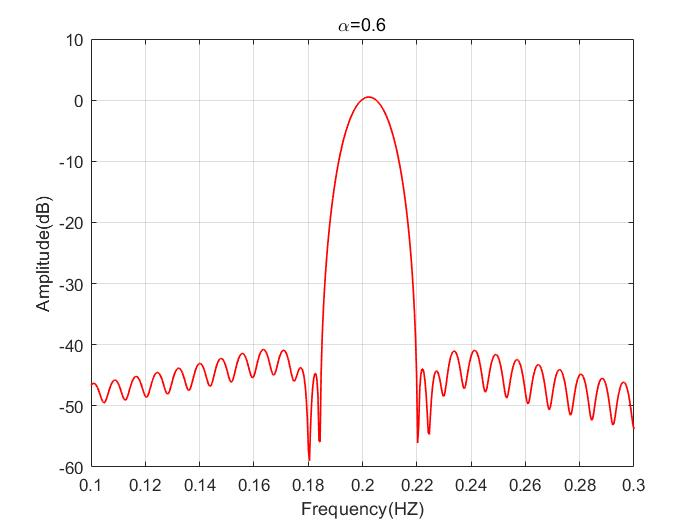
\includegraphics[width=7.5cm]{2/ham06.jpg}
    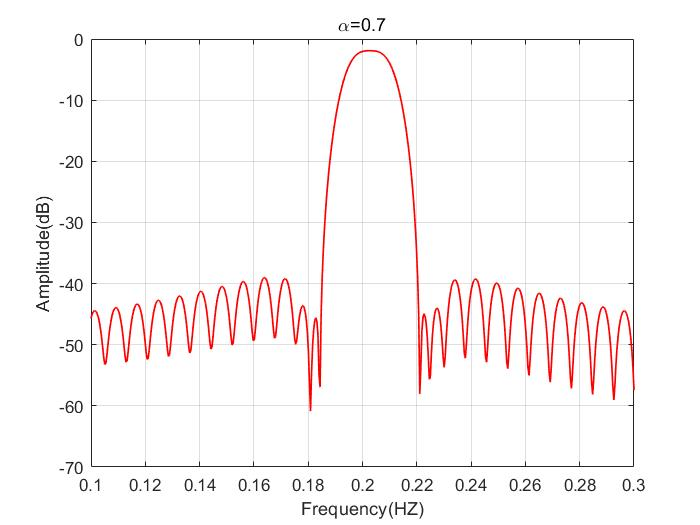
\includegraphics[width=7.5cm]{2/ham07.jpg}
    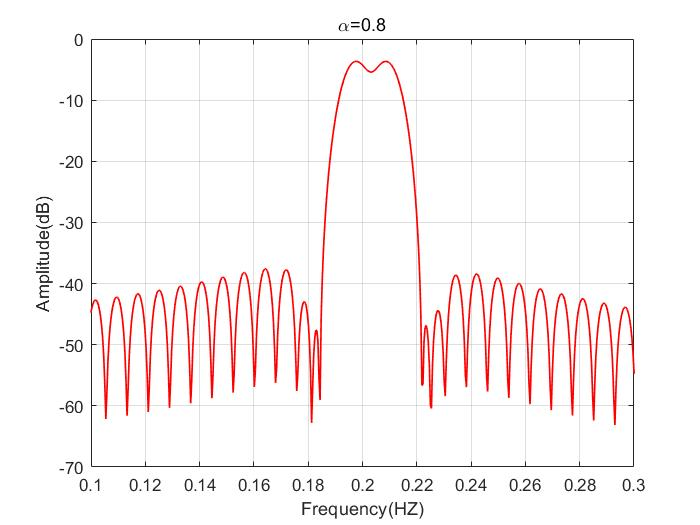
\includegraphics[width=7.5cm]{2/ham08.jpg}
    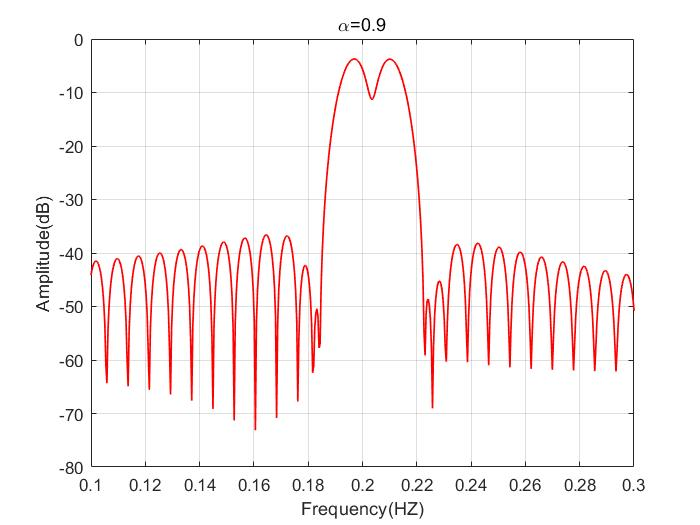
\includegraphics[width=7.5cm]{2/ham09.jpg}
    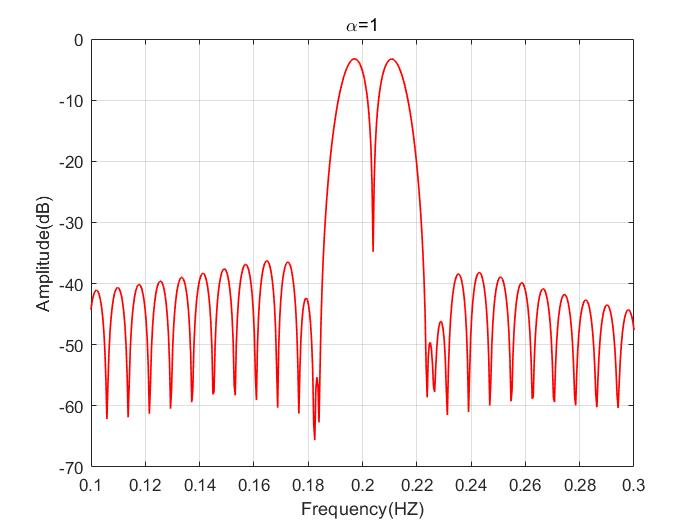
\includegraphics[width=7.5cm]{2/ham10.jpg}
    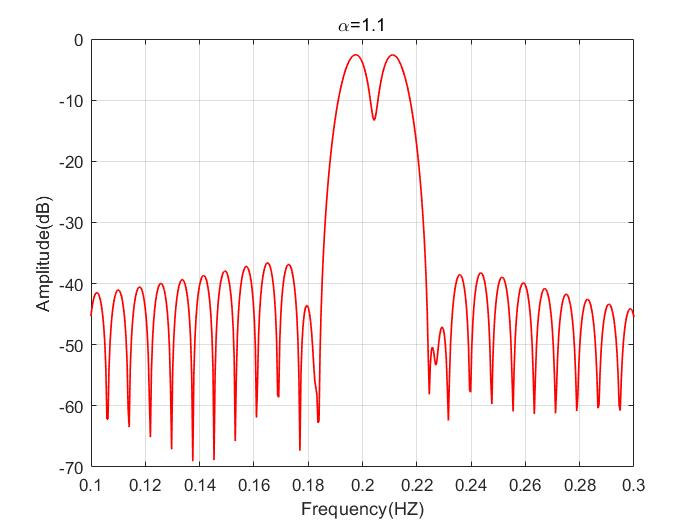
\includegraphics[width=7.5cm]{2/ham11.jpg}
    \caption{$\alpha= 0.6, 0.7, 0.8, 0.9, 1.0,1.1$}
\end{figure}

We see the threshold $\alpha $ is about 0.8 in this case, due to the slightly wider main lobe width
of the Hamming window, in comparison to the Bartlett window.
\subsubsection{The Solution of (d)}
We have the result of the experiment:
\begin{figure}[htbp]
    \centering
    
    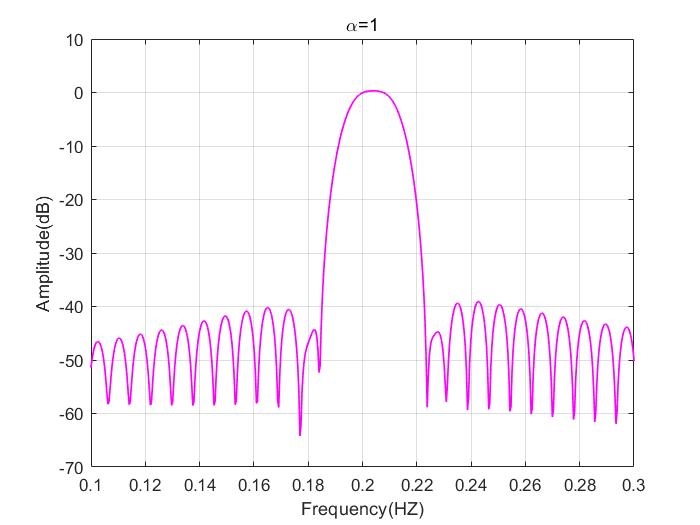
\includegraphics[width=7.5cm]{2/b10.jpg}
    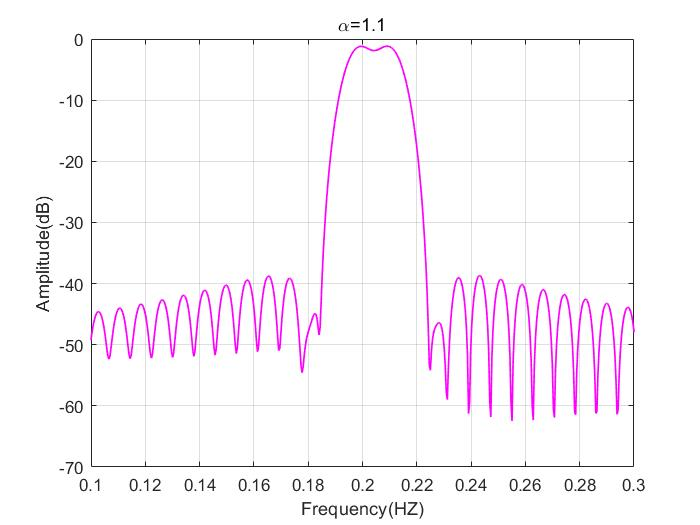
\includegraphics[width=7.5cm]{2/b11.jpg}
    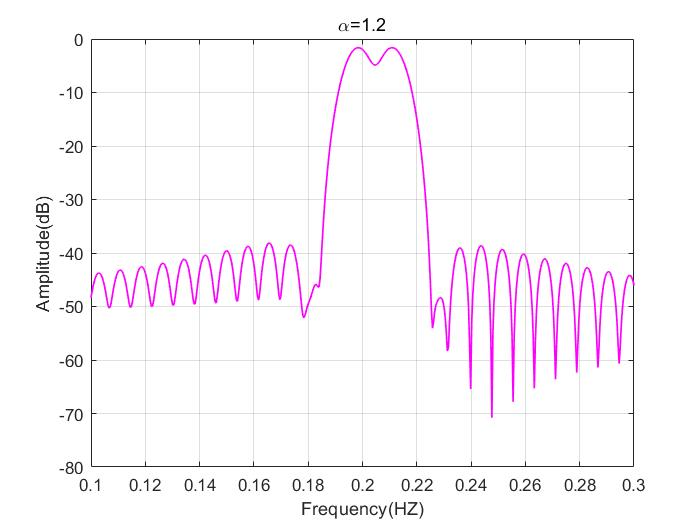
\includegraphics[width=7.5cm]{2/b12.jpg}
    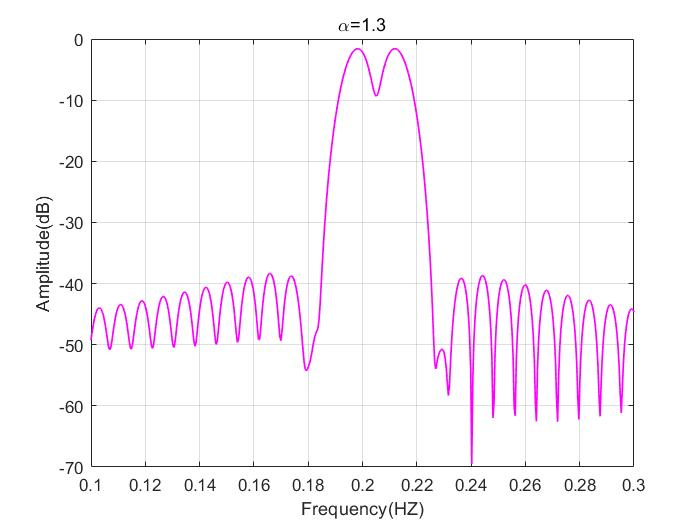
\includegraphics[width=7.5cm]{2/b13.jpg}
    \caption{$\alpha=  1.0,1.1,1.2,1.3$ and $\phi_1=0, \phi_2=30$}
\end{figure}

When the signals are out of phase, we obtain the above plots (in comparison to part (b) when $ \phi_1 = \phi_2 = 0$); we see that the threshold $\alpha$ is about 1.1 for this case.


We can also test different amplitudes and noise variances to verify that the resolution does not change much as these parameters change; one such result (for $a_1 = 10$, $a_2 = 5$, $\phi_1 = \phi_2 = 0$, and $\sigma^2 = 1$) is shown below.
\begin{figure}[htbp]
    \centering
    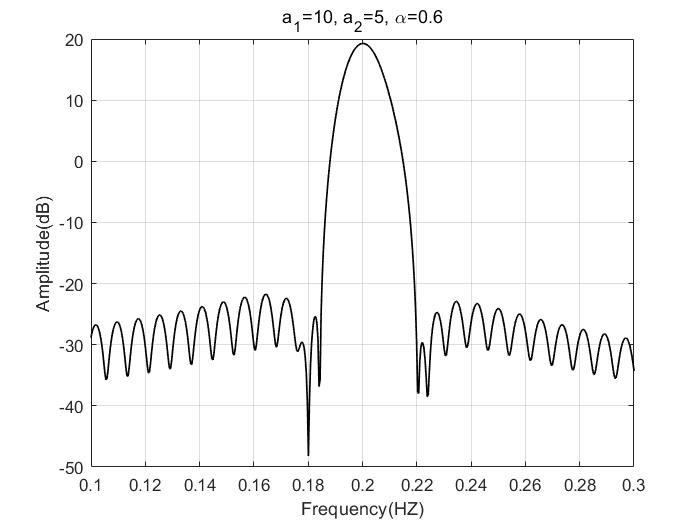
\includegraphics[width=7.5cm]{2/dd06.jpg}
    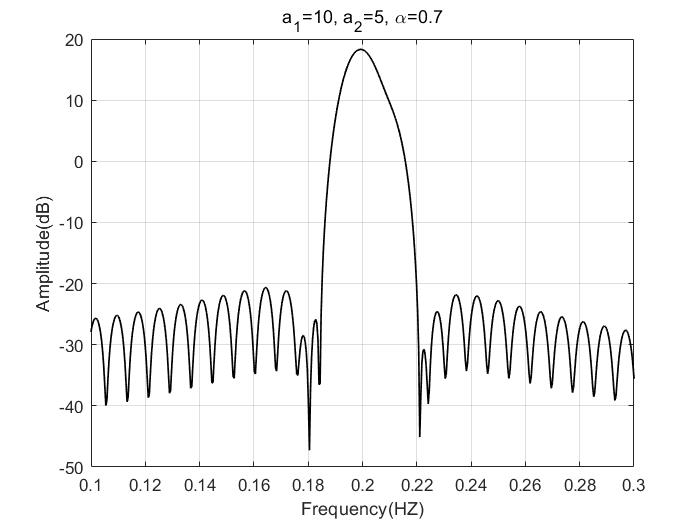
\includegraphics[width=7.5cm]{2/dd07.jpg}
    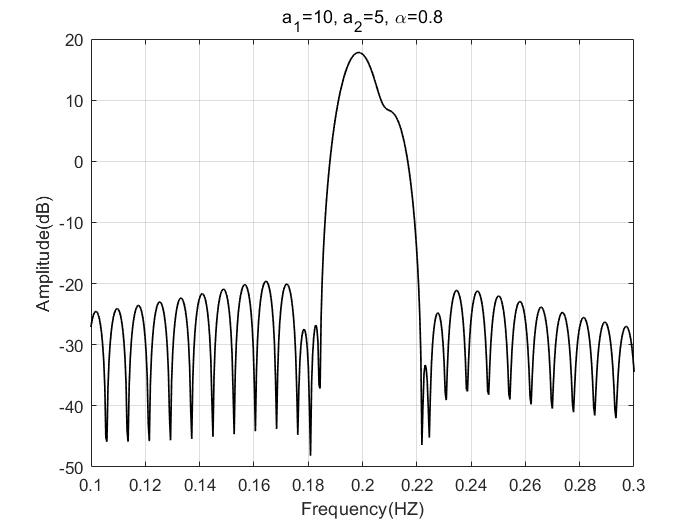
\includegraphics[width=7.5cm]{2/dd08.jpg}
    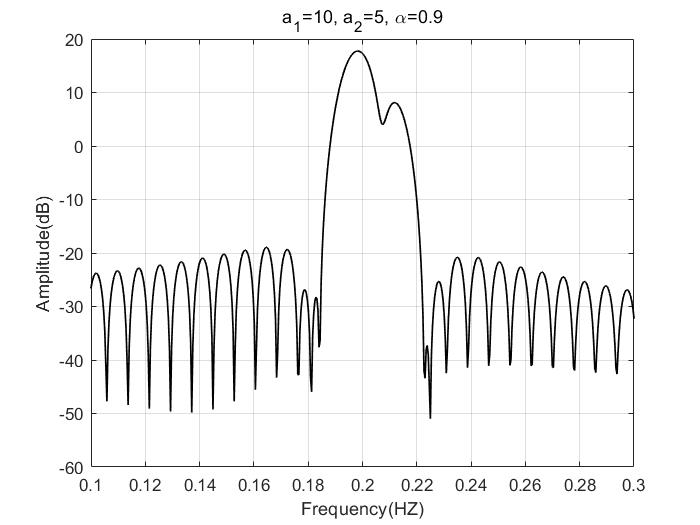
\includegraphics[width=7.5cm]{2/dd09.jpg}
    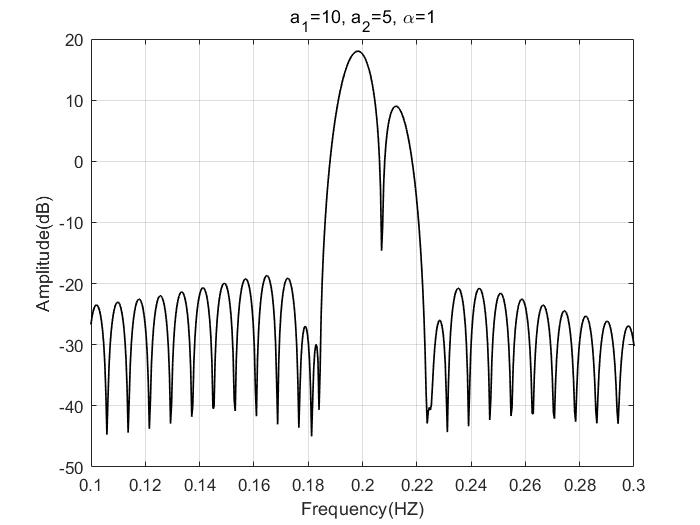
\includegraphics[width=7.5cm]{2/dd10.jpg}
    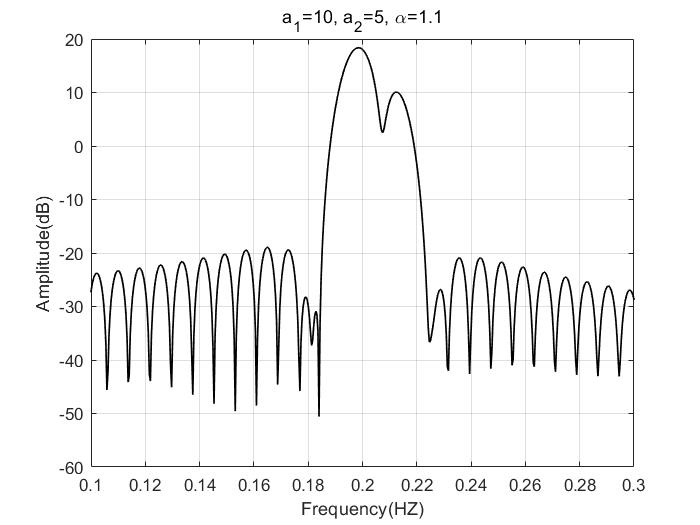
\includegraphics[width=7.5cm]{2/dd11.jpg}
    \caption{$\alpha=  0.6,0.7,0.8,0.9,1.0,1.1$ and $\phi_1=\phi_2=0$ and $a_1=10, a_2=5$}
\end{figure}

\subsection{Spectral Leakage}
\subsubsection{The Solution of (a)}
When $\alpha=4$, we have the result of the experiment:
\begin{figure}[htbp]
    \centering
    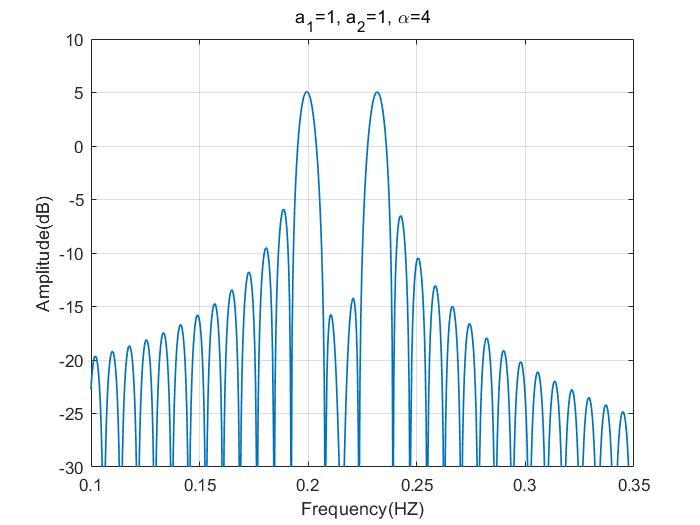
\includegraphics[width=7.5cm ]{2/ea1.jpg}
    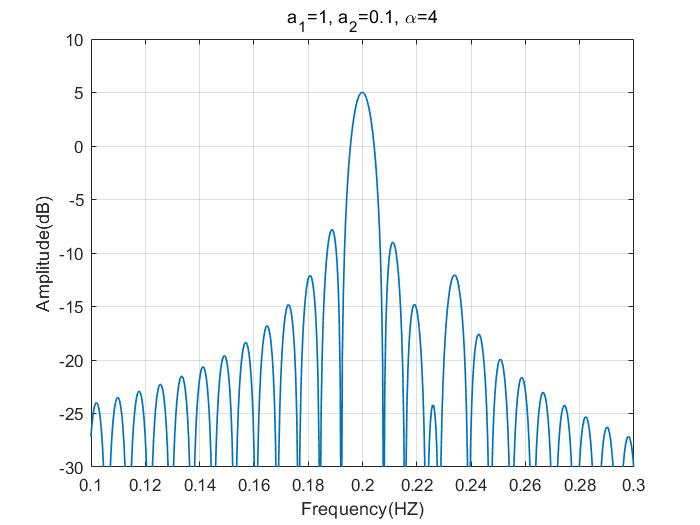
\includegraphics[width=7.5cm ]{2/ea2.jpg}
    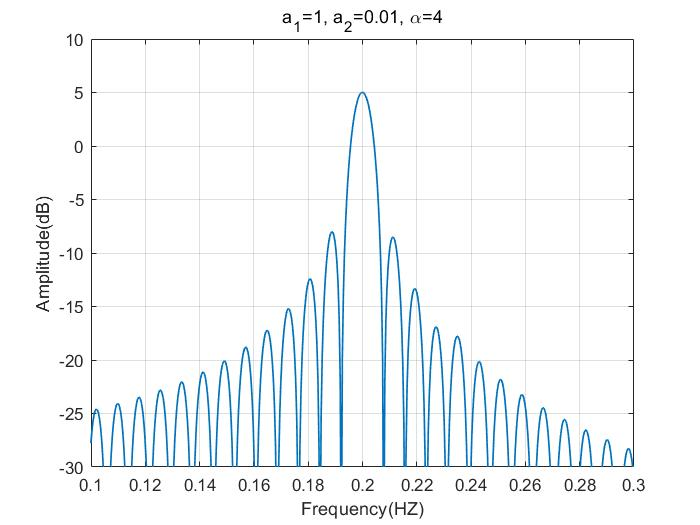
\includegraphics[width=7.5cm ]{2/ea3.jpg}
    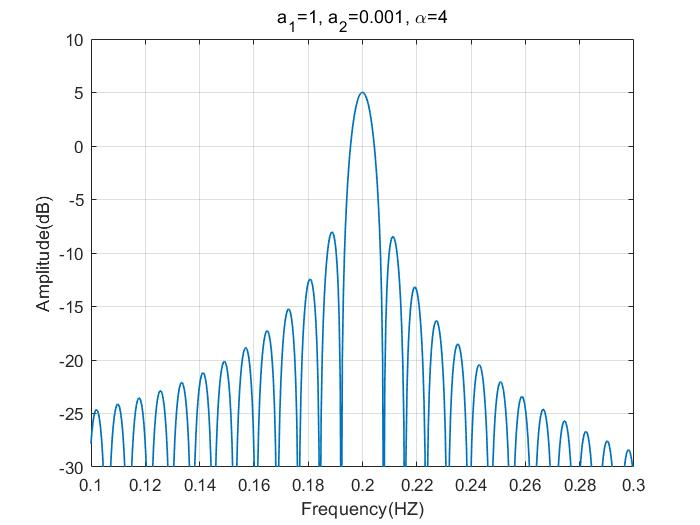
\includegraphics[width=7.5cm ]{2/ea4.jpg}
    \caption{$\alpha=4$ and $a_1=1, a_2=1, 0.1,0.01,0.001$, respectively}
\end{figure}

We see that, because of window leakage, the weaker sinusoidal component can be detected when $a_2 = 0.1$, but not for $a_2 = 0.01$.\newpage

\subsubsection{The Solution of (b)}
When $\alpha=12$, we have the result of the experiment:
\begin{figure}[htbp]
    \centering
    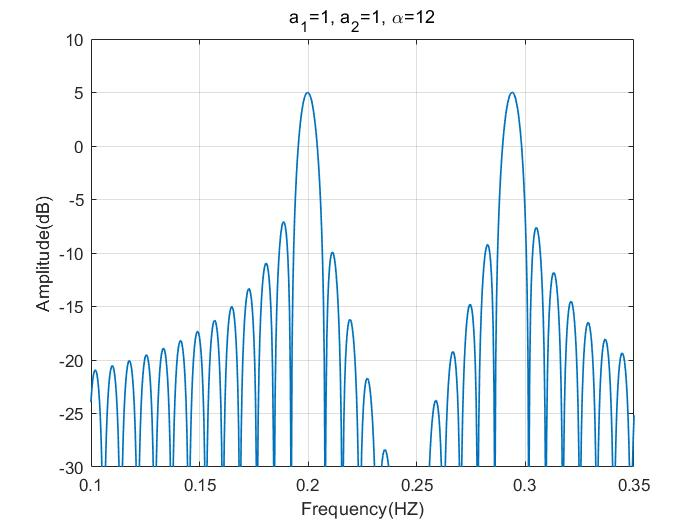
\includegraphics[width=7.5cm ]{2/ea5.jpg}
    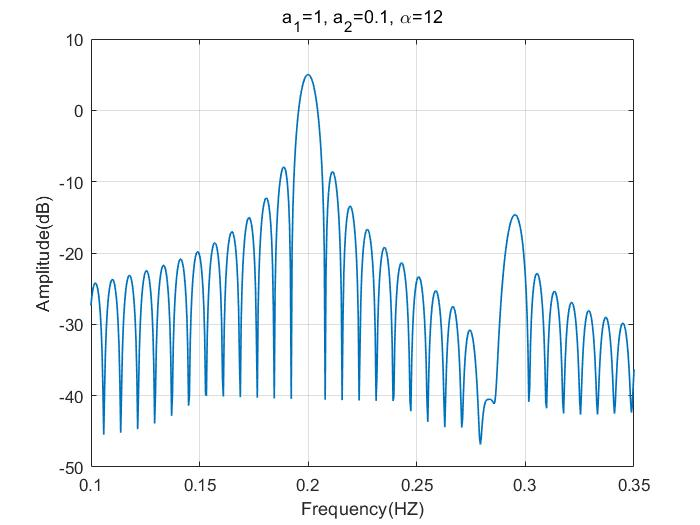
\includegraphics[width=7.5cm ]{2/ea6.jpg}
    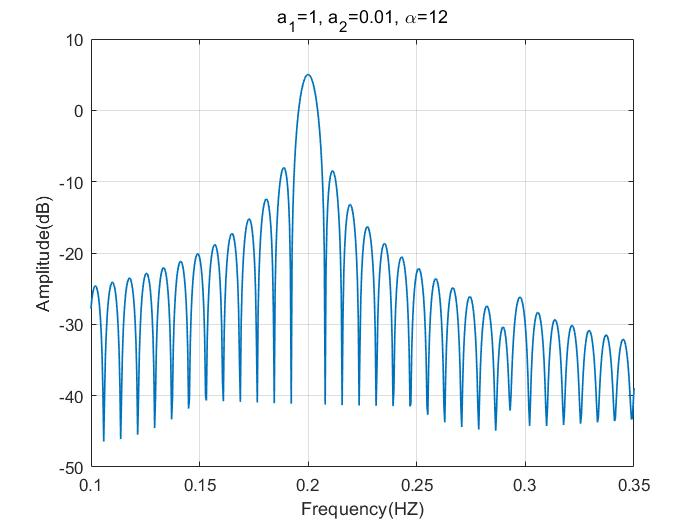
\includegraphics[width=7.5cm ]{2/ea7.jpg}
    \includegraphics[width=7.5cm ]{2/ea8.jpg}
    \caption{$\alpha=12$ and $a_1=1, a_2=1, 0.1,0.01,0.001$, respectively}
\end{figure}

We see that, because of window leakage, the weaker sinusoidal component can be detected when $a_2 = 0.01$, but not for $a_2 = 0.001$.
\subsubsection{The Solution of (c)}

The mean of the estimated spectrum will be the true spectrum convolved with the Bartlett window. Thus, sidelobes of the stronger sinusoid peak, after convolution, may be larger than the main lobe level of the weaker sinusoid peak, if the weaker sinusoid is sufficiently weak. The sidelobe level for the Bartlett window is about -35dB at $\alpha= 4$ (4 Fourier resolution bins), and about -50dB for $\alpha = 12$. For $\alpha = 4 $ we could detect a weaker sinusoid whose power is 20dB below a stronger sinusoid power, but not when the weaker sinusoid power is 40dB below; this is consistent with the -35dB sidelobe level. Similar comments apply for $\alpha = 12$.
\subsubsection{The Solution of (d)}
We have the result of the experiment:
\begin{figure}[htbp]
    \centering
    \includegraphics[width=12cm]{2/window.jpg}
    \caption{The Chebwin Window Frequency Response}
\end{figure}
\begin{figure}[htbp]
    \centering
    \includegraphics[width=12cm]{2/windowed.jpg}
    \caption{Windowed Peroidogram Estimation}
\end{figure}

We show results above for N = 128, although the results are essentially independent of N since the frequency separation is also a function of N. From the Chebyshev window we see the main lobe width is about $\frac{4.9}{N}$; when we set the second frequency at -50 dB and using $\alpha=\frac{4.9}{N}$, we obtain the windowed periodogram result above, and we see that we can indeed detect the weaker sinusoid. Note that a plot of $20\log_{10} |V (\omega)/V (0)|$ is the same as the top figure above, since $W(\omega) = |V (\omega)|^2$. The Blackman–Tukey method fails because its mean spectrum is, from equations (2.5.3) and (2.4.8), the convolution of the true spectrum, the Bartlett window, and the Chebyshev window. Even though the Chebyshev window has low sidelobes, the Bartlett window does not, and the weak sinusoid cannot be detected.
\end{document}